\documentclass{beamer}
\usetheme{Madrid}
\usecolortheme{default}

\usepackage{physics}
\usepackage{graphicx}

\title{Cavity Blockade in the Jaynes-Cummings Model}
\author{Álvaro Méndez}
\institute{DFA UniPD}
\date{February 16, 2026}

\begin{document}

% SLIDE 1: Title
\begin{frame}
  \titlepage
\end{frame}

% SLIDE 2: Model and Hamiltonian
\begin{frame}{The Driven Jaynes-Cummings Model}
  The system consists of a two-level atom coupled to a cavity mode, driven by an external laser field $\mathcal{E}$.
  \vfill
  \textbf{Rotating Frame Hamiltonian (RWA):}
  \begin{equation*}
    H' = \delta_c a^\dagger a + \delta_a \ket{e}\bra{e} + g(\sigma^+ a + \sigma^- a^\dagger) + \mathcal{E}(a + a^\dagger)
  \end{equation*}
  \vfill
  \textbf{Physical Meaning of $H_d$:}
  \begin{itemize}
    \item Represents a \textbf{coherent driving field} pumping the cavity.
    \item Realized experimentally by a laser beam of frequency $\omega$.
    \item $\mathcal{E}$ characterizes the laser intensity/amplitude.
  \end{itemize}
\end{frame}

% SLIDE 3: Non-Coupled Case (g=0)
\begin{frame}{Linear Regime: The Coherent State ($g=0$)}
  In the absence of atom-cavity coupling, the system behaves as a driven damped harmonic oscillator.
  \begin{columns}
    \begin{column}{0.5\textwidth}
      \begin{itemize}
        \item Steady state is a \textbf{coherent state} $|\alpha\rangle$.
        \item Occupation follows a \textbf{Poisson distribution}.
      \end{itemize}
    \end{column}
    \begin{column}{0.5\textwidth}
      \centering
      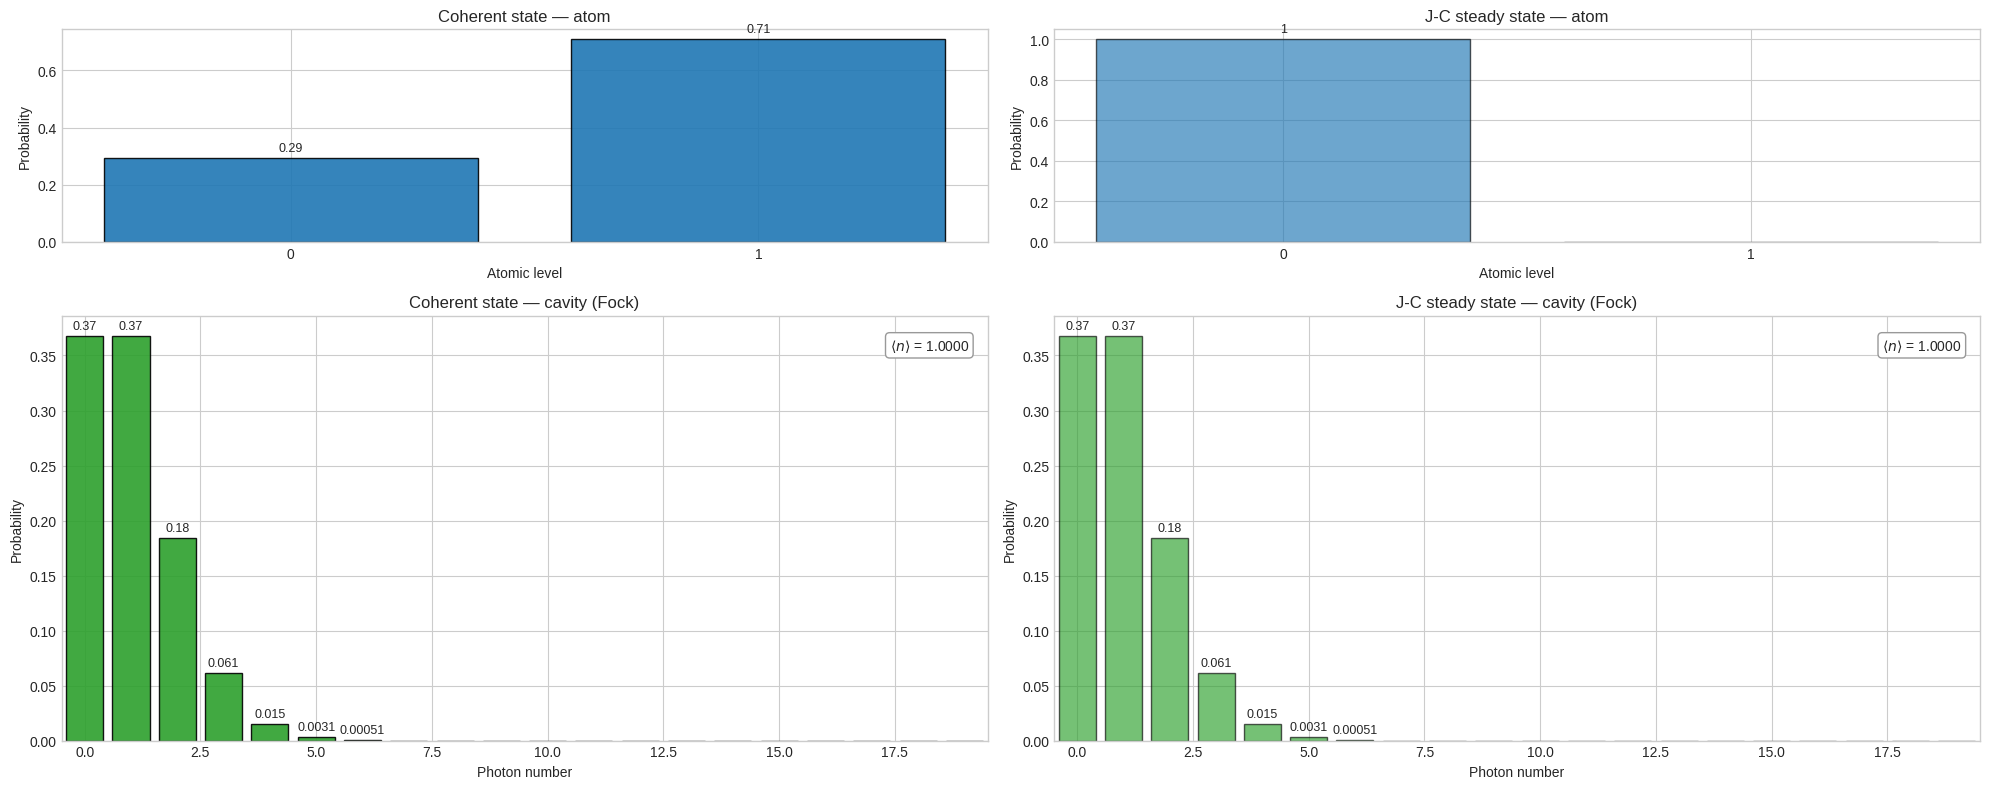
\includegraphics[width=\textwidth]{hist_no_g.png}
      \textit{Result:} Distribution matches the analytical Poissonian curve.
    \end{column}
  \end{columns}
\end{frame}

% SLIDE 4: Strong Coupling & The Blockade
\begin{frame}{The Photon Blockade Effect}
  In the strong coupling regime ($g \gg \kappa, \Gamma$), the J-C ladder becomes \textbf{anharmonic}.
  
  \begin{itemize}
    \item \textbf{Mechanism:} Tuning $\omega$ to the first polariton resonance ($\omega_c \pm g$) allows one photon to enter the cavity.
    \item \textbf{The Block:} The transition to the 2-photon state is detuned by $(\sqrt{2}-1)g$, preventing multi-photon absorption.
  \end{itemize}
  \centering
  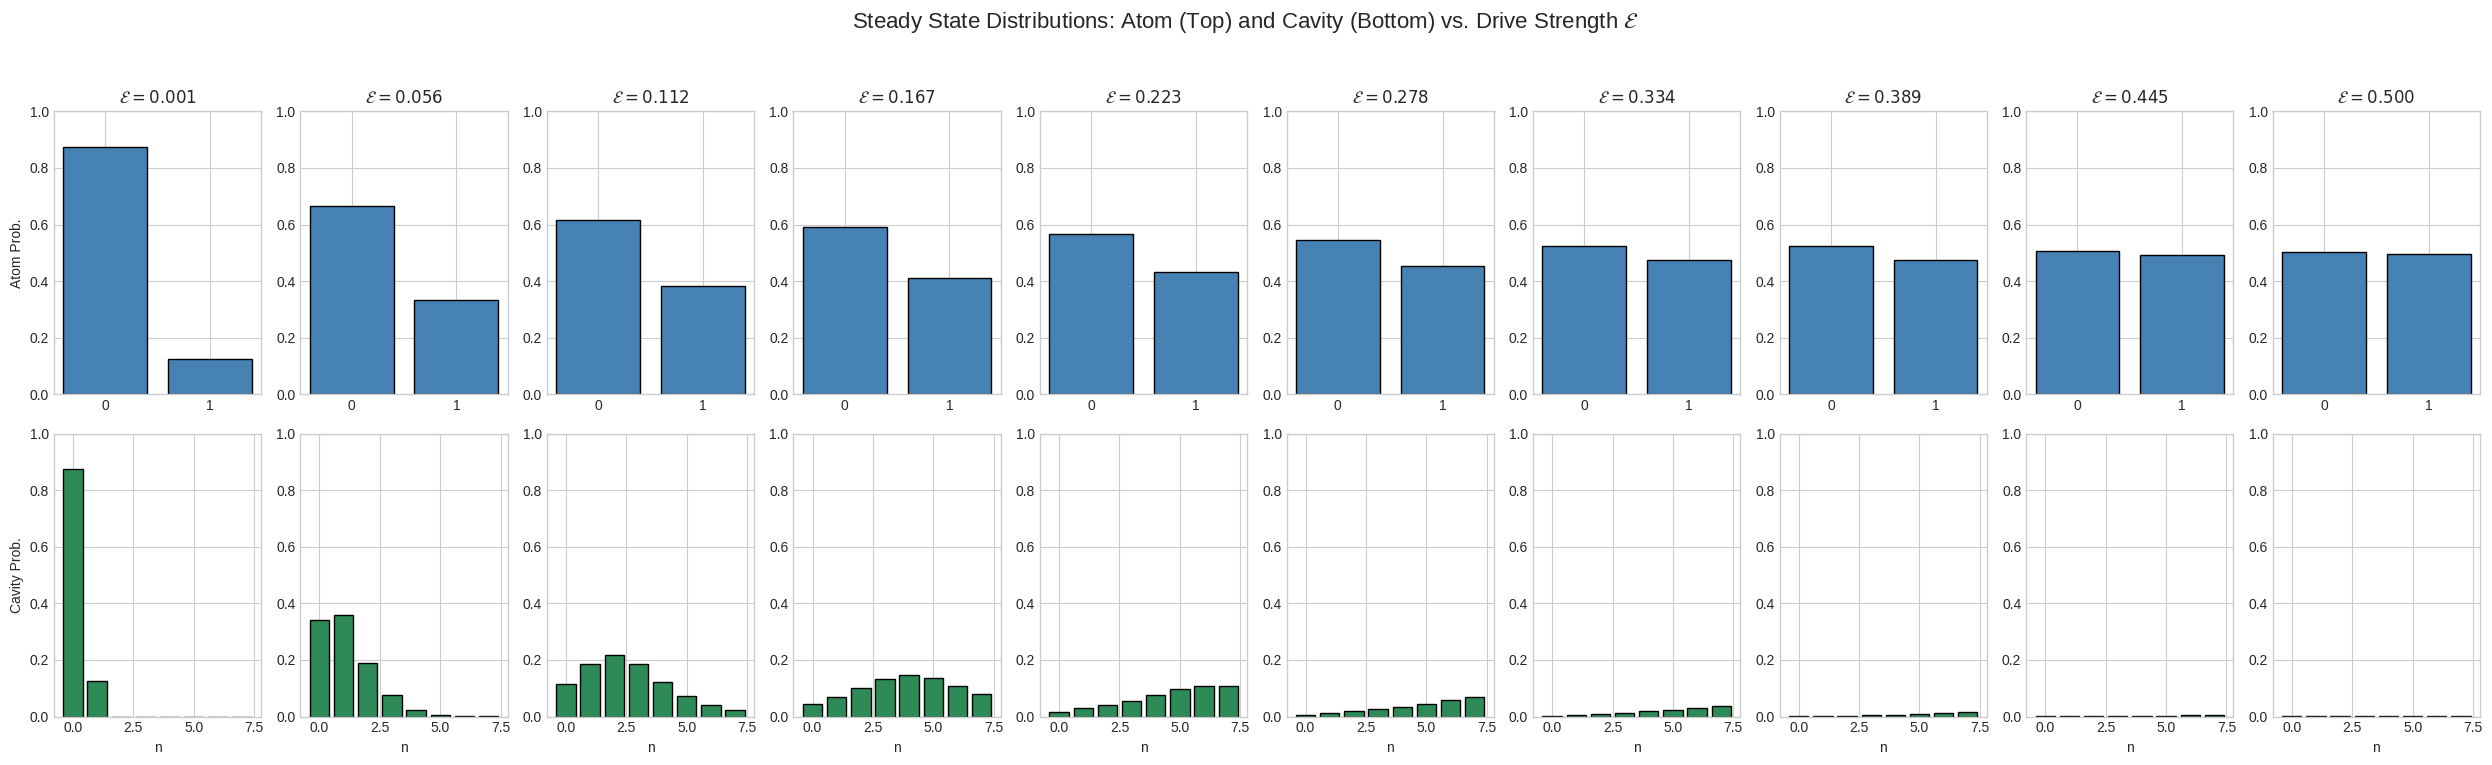
\includegraphics[width=0.6\textwidth]{E_prob_strong.png}
  \textit{Observation:} $P(n \ge 2)$ remains negligible even as drive $\mathcal{E}$ increases.
\end{frame}

% SLIDE 5: Parameter Sensitivity (g, kappa, Gamma)
\begin{frame}{Sensitivity to Dissipation and Coupling}
  \begin{columns}
    \begin{column}{0.5\textwidth}
      \textbf{Coupling $g$:}
      \begin{itemize}
        \item Larger $g$ increases anharmonicity and improves blockade quality.
      \end{itemize}
      \textbf{Dissipation $\kappa, \Gamma$:}
      \begin{itemize}
        \item Increasing decay rates broadens peaks.
        \item Is harder to keep photons in the cavity, reducing blockade effectiveness.
      \end{itemize}
    \end{column}
    \begin{column}{0.5\textwidth}
      \centering
      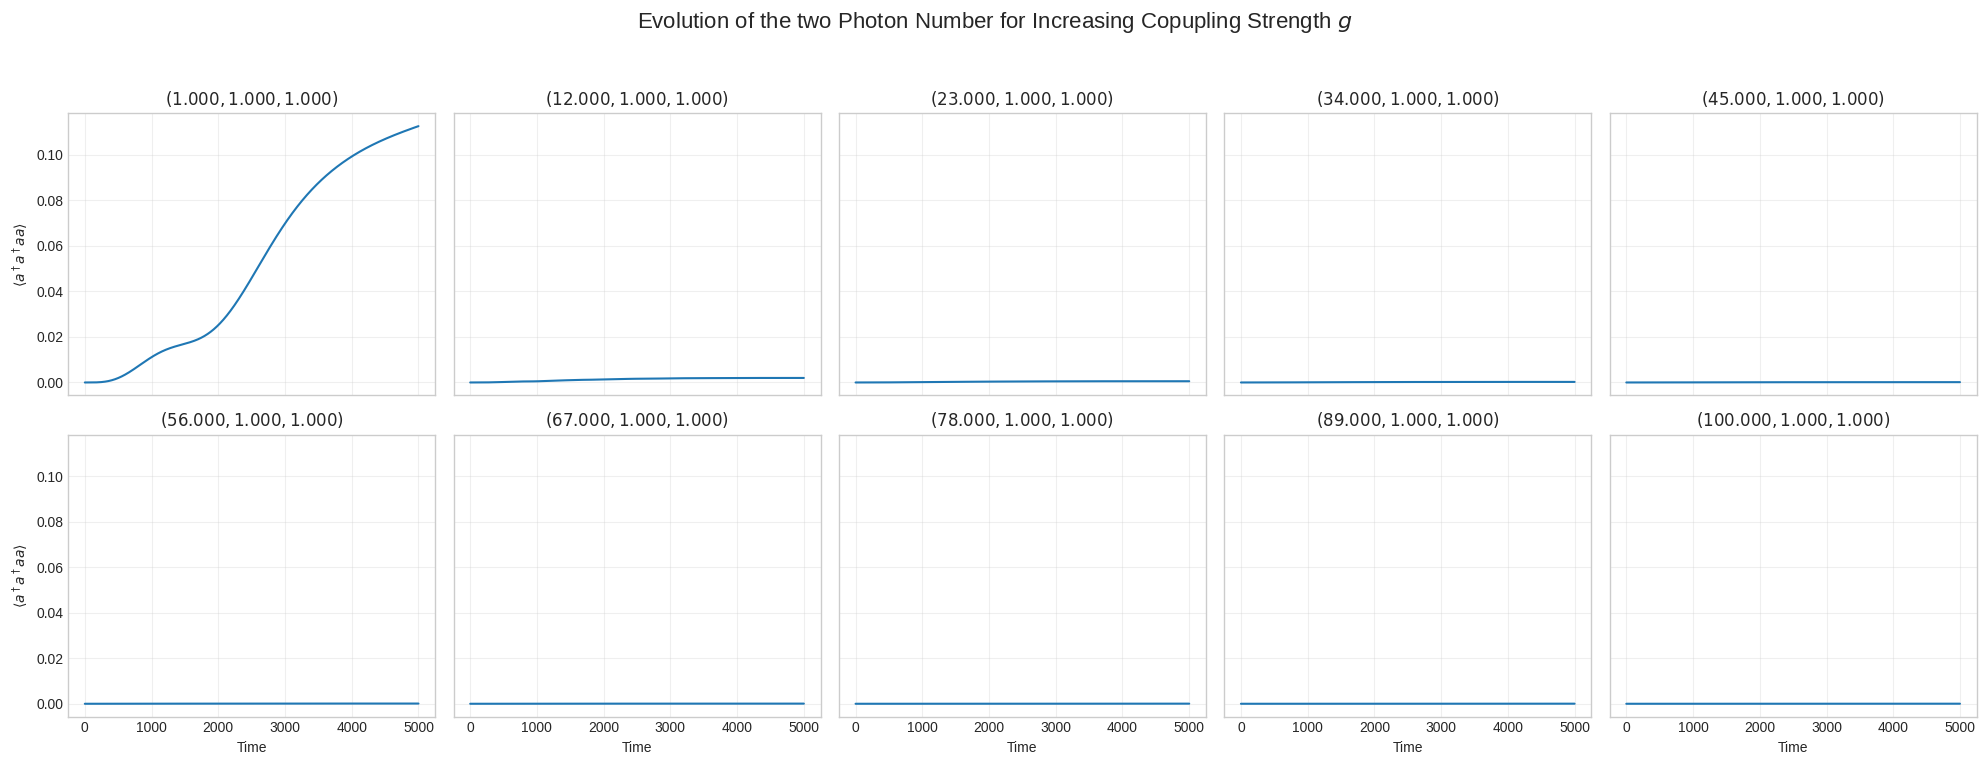
\includegraphics[width=\textwidth]{g_epxect_strong.png}
      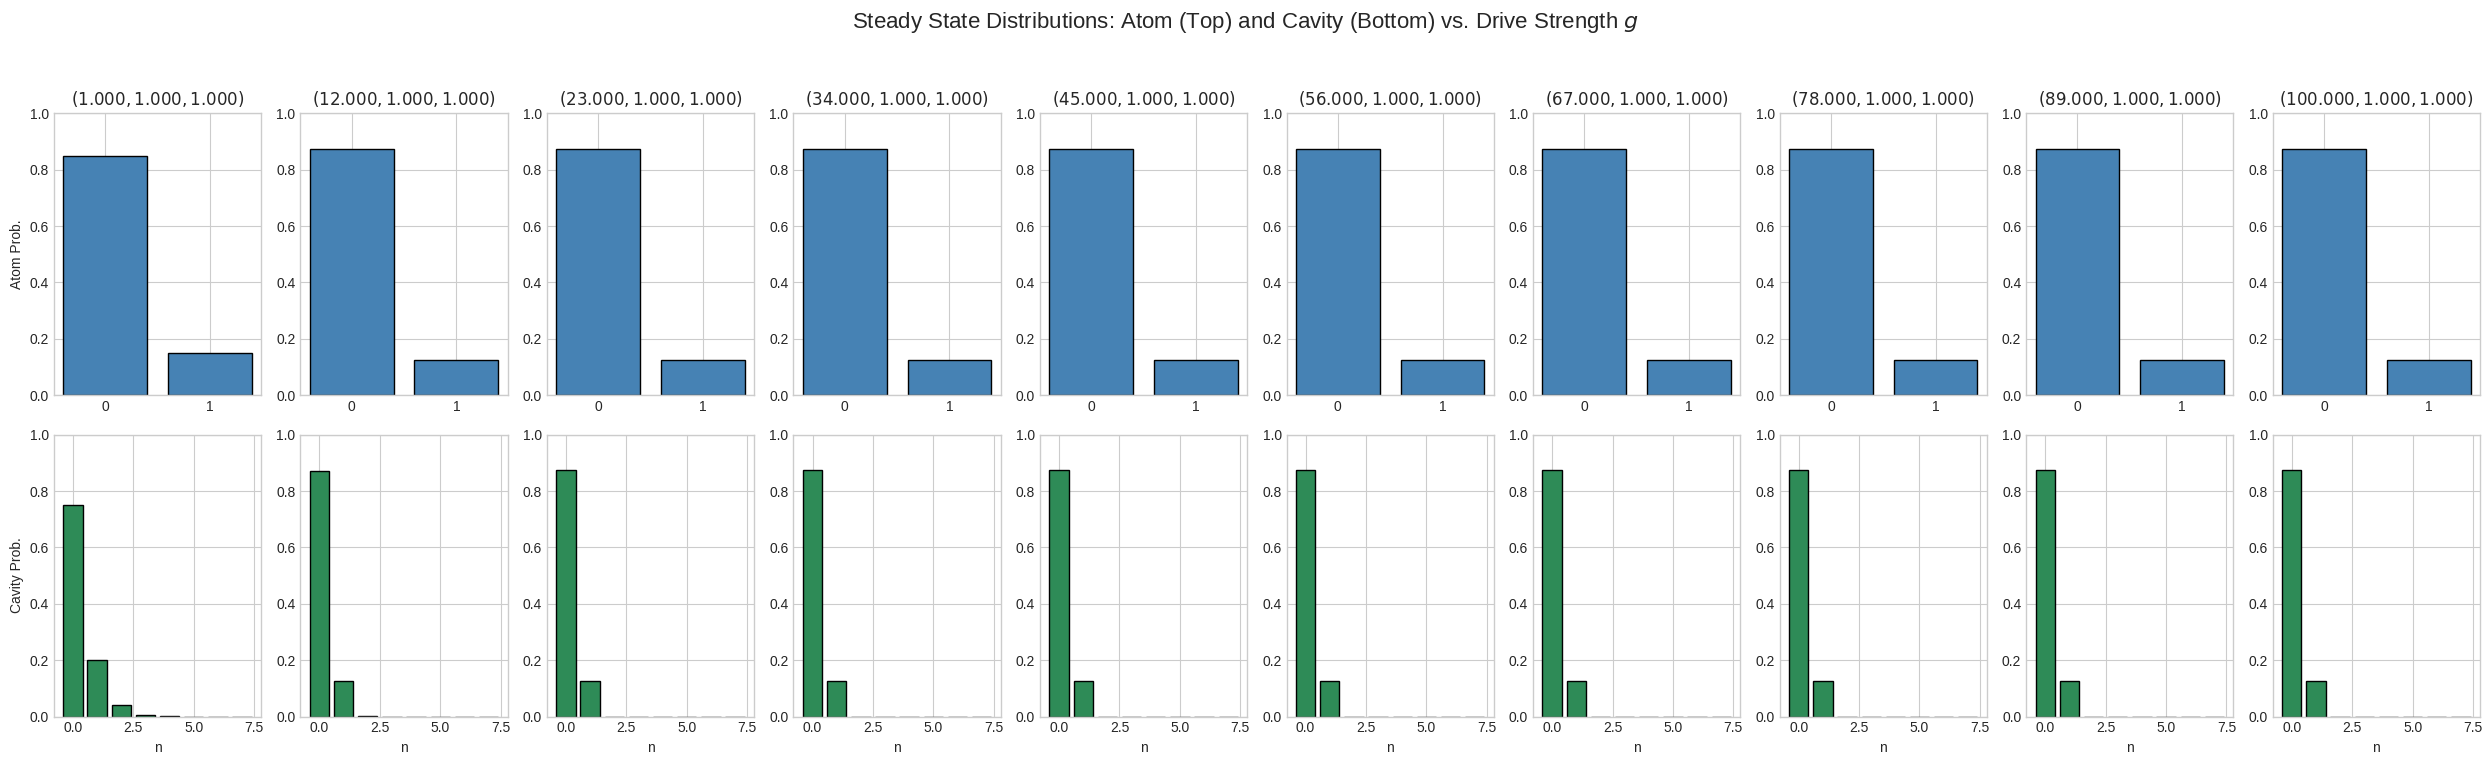
\includegraphics[width=\textwidth]{g_prob_strong.png}
      \vfill
      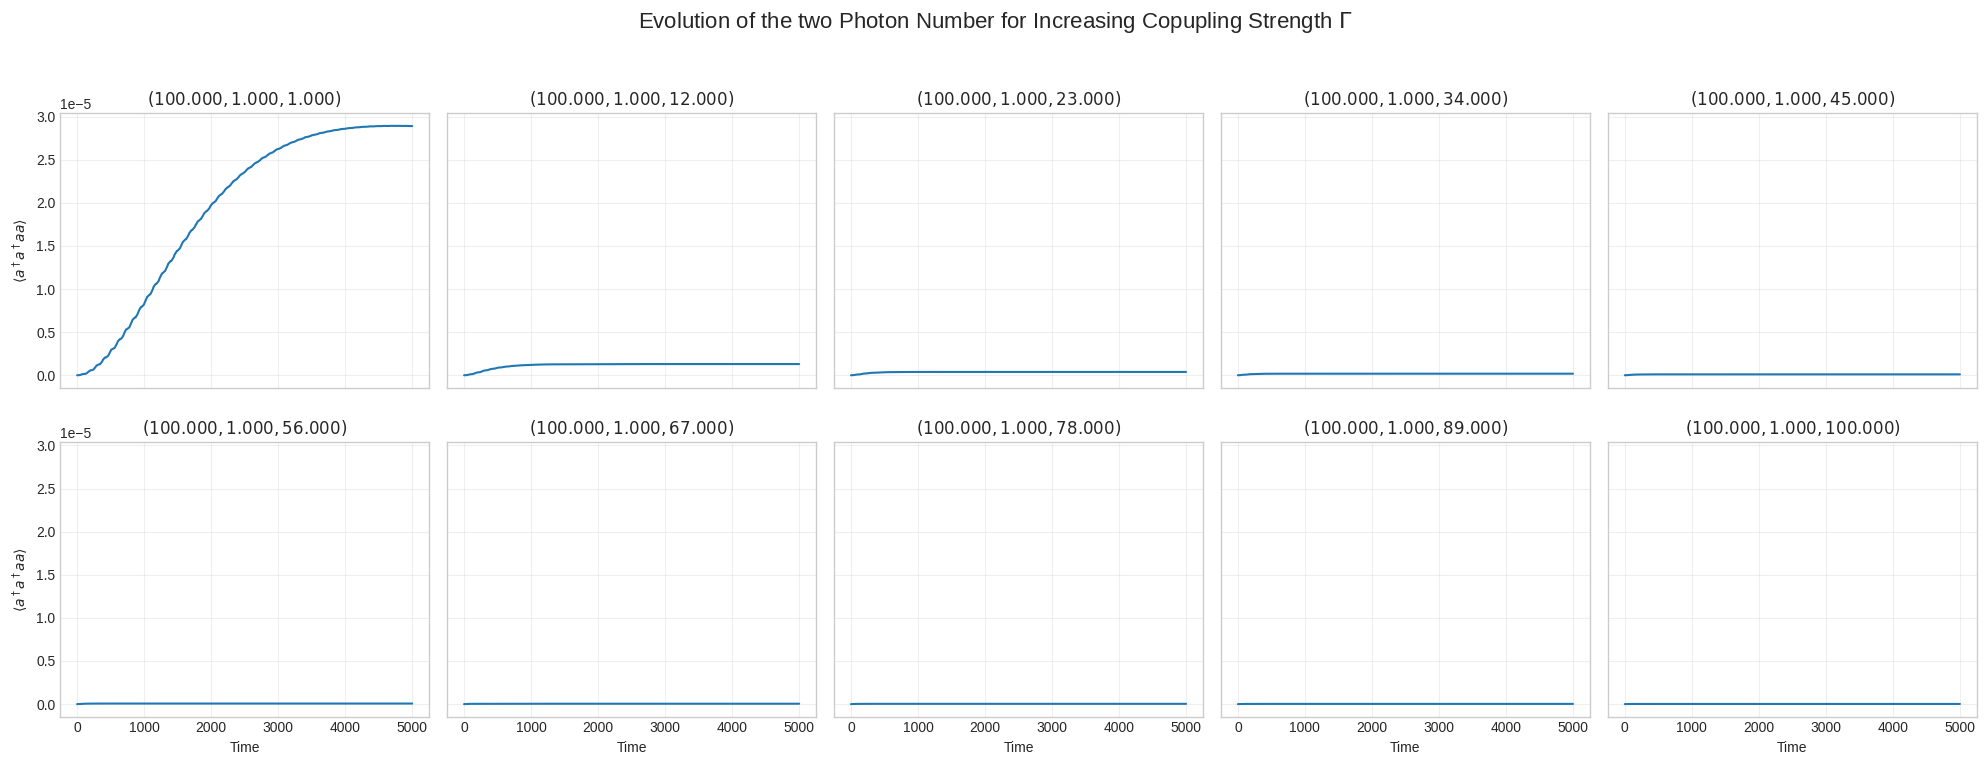
\includegraphics[width=\textwidth]{G_epxect_strong.png}
      \textit{Analysis:} Low $\kappa$ is essential for resolved quantum states.
    \end{column}
  \end{columns}
\end{frame}

% SLIDE 6: Photon Statistics: $g^{(2)}(0)$
\begin{frame}{Quantifying the Blockade: $g^{(2)}(0)$}
  The second-order correlation function measures the probability of detecting two simultaneous photons.
  \begin{equation*}
    g^{(2)}(0) = \frac{\langle a^\dagger a^\dagger a a \rangle}{\langle a^\dagger a \rangle^2}
  \end{equation*}
  \vfill
  \textbf{Numerical Results ($g=100$):}
  \begin{itemize}
    \item $\langle n \rangle \approx 0.125$
    \item $g^{(2)}(0) \approx 0.0018$
  \end{itemize}
  \vfill
  \textbf{Conclusion:} $g^{(2)}(0) \ll 1$ confirms it. The field is a source of single photons.
\end{frame}

% SLIDE 7: Vacuum Rabi Splitting
\begin{frame}{Spectroscopy: Vacuum Rabi Splitting}
  Scanning the drive frequency $\omega$ reveals the dressed states of the system.
  \centering
  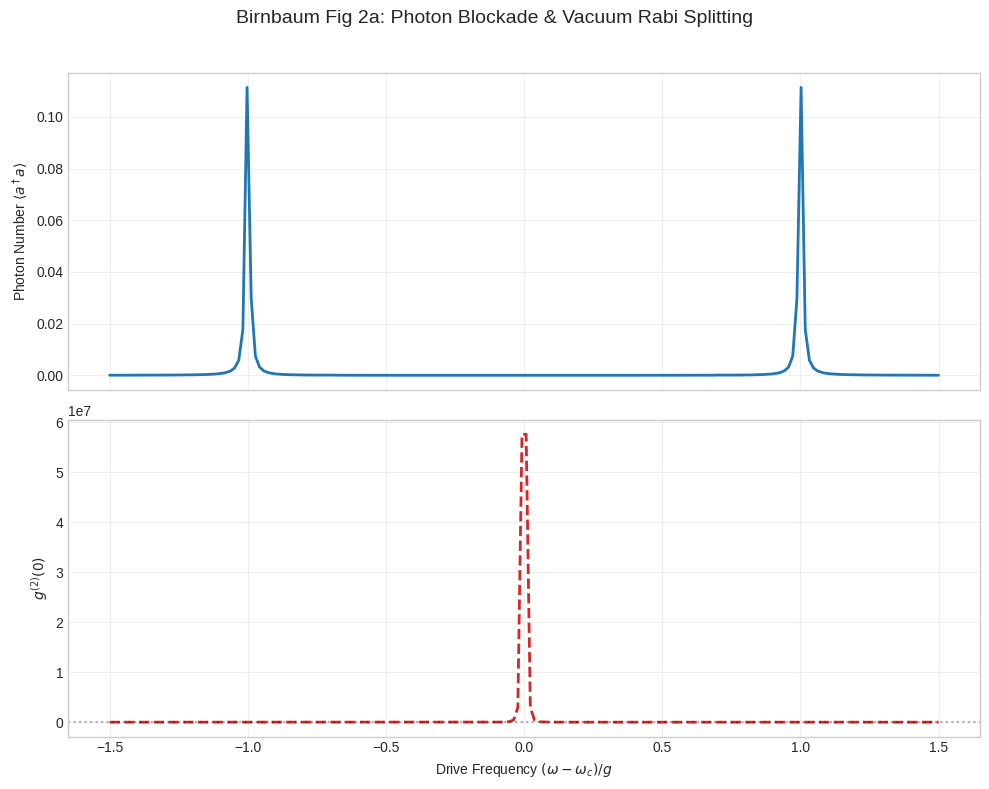
\includegraphics[width=0.6\textwidth]{B.png}
  \vfill
  \begin{itemize}
    
    \item Matches experimental results (e.g., Birnbaum et al.).
    
  \end{itemize}
\end{frame}

\end{document}